\section{Hinweise zur Umsetzung}
Die folgenden Mockups dienen der visuellen Vorstellung einiger der wichtigsten Moderator- und Benutzerprozesse in der vorgesehenen Software. Spezifische optische und funktionale Details können sich während des Entwicklungsprozesses je nach Kundenwunsch ändern.
\linebreak
\linebreak

\begin{figure}[h]
  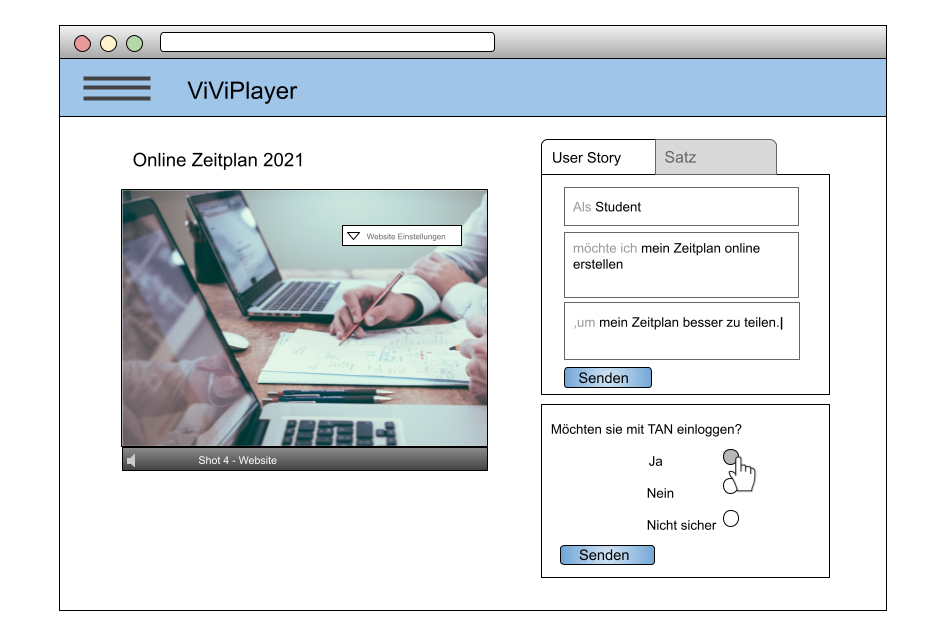
\includegraphics[width=\linewidth]{5dot1.png}
  \caption{Hier sieht man den ViViPlayer aus der Perspektive des Benutzers. Der Nutzer hat die Möglichkeit, strukturierte User-Stories oder Freitextsätze zu senden. Vom Moderator gestellte Fragen können direkt beantwortet werden. Der Videoplayer ermöglicht es dem Benutzer, das Video anzusehen, ohne die Wiedergabe für andere Teilnehmer zu stören. Vom Moderator bereitgestellte Annonatation können geöffnet und geschlossen werden.}
  \label{fig:5dot1}
\end{figure}

\begin{figure}
  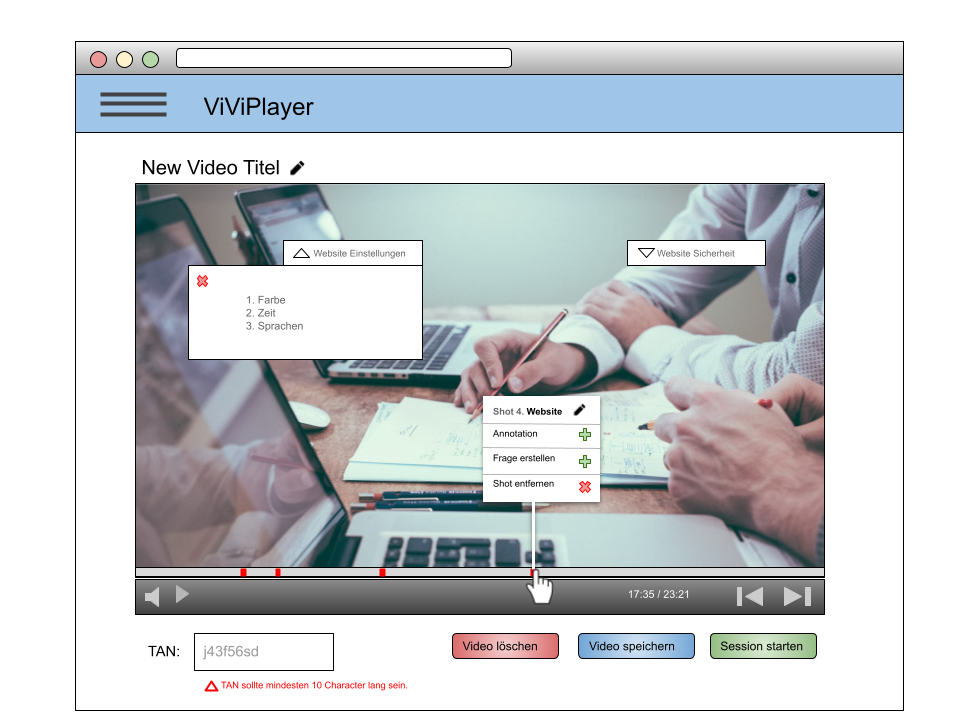
\includegraphics[width=\linewidth]{5dot2.png}
  \caption{Abbildung 2. Hier kann man sehen, wie ein neues Video für eine neue Sitzung von einem Moderator bearbeitet wird. Das Video wurde bereits automatisch in Kapitel unterteilt. Der Titel des Videos kann direkt geändert werden. Der Moderator hat die Möglichkeit, Kapitel und Annonatation hinzuzufügen und zu entfernen sowie jedem Kapitel Titel zuzuordnen und Fragen vorzuformulieren, indem er einfach auf die Segmente auf dem Video-Slider klickt. Wenn der Moderator mit dem Video zufrieden ist, kann er eine TAN vergeben und das Video entweder speichern oder direkt eine Live-Session starten.}
  \label{fig:5dot2}
\end{figure}

\begin{figure}
  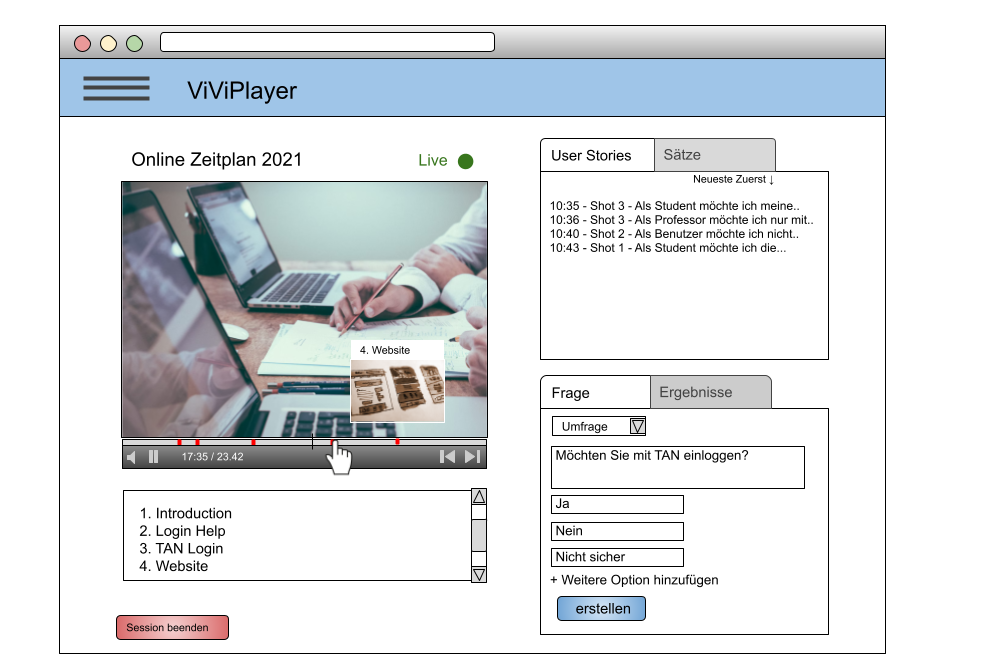
\includegraphics[width=\linewidth]{5dot3.png}
  \caption{Abbildung 3. Hier sieht man eine Live-Session aus der Sicht des Moderators. Im Gegensatz zur der Perspektive des Benutzers, hat der Moderator die volle Kontrolle über die Navigation des Videoplayers. Der Moderator hat die Möglichkeit, zu jedem gewünschten Teil des Videos zu springen. Zusätzliche Schaltflächen erleichtern es dem Moderator, zum Anfang oder Ende eines Kapitels zu springen. Der Moderator hat die Möglichkeit, Antworten von Benutzern zu lesen, sobald sie eintreffen. Dazu gehören User Stories, Sätze und Umfrageergebnisse.}
  \label{fig:5dot3}
\end{figure}

